%% Run LaTeX on this file several times to get Table of Contents,
%% cross-references, and citations.

\documentclass[11pt]{book}
\usepackage{gvv-book}
%\usepackage{Wiley-AuthoringTemplate}
\usepackage[sectionbib,authoryear]{natbib}% for name-date citation comment the below line
%\usepackage[sectionbib,numbers]{natbib}% for numbered citation comment the above line
\def\inputGnumericTable{}
\usepackage{array}
\usepackage{longtable}
\usepackage{calc}
\usepackage{multirow}
\usepackage{hhline}
\usepackage{ifthen}

%%********************************************************************%%
%%       How many levels of section head would you like numbered?     %%
%% 0= no section numbers, 1= section, 2= subsection, 3= subsubsection %%
\setcounter{secnumdepth}{3}
%%********************************************************************%%
%%**********************************************************************%%
%%     How many levels of section head would you like to appear in the  %%
%%				Table of Contents?			%%
%% 0= chapter, 1= section, 2= subsection, 3= subsubsection titles.	%%
\setcounter{tocdepth}{2}
%%**********************************************************************%%

%\includeonly{ch01}
\makeindex

\begin{document}

\frontmatter
%%%%%%%%%%%%%%%%%%%%%%%%%%%%%%%%%%%%%%%%%%%%%%%%%%%%%%%%%%%%%%%%
%% Title Pages
%% Wiley will provide title and copyright page, but you can make
%% your own titlepages if you'd like anyway
%% Setting up title pages, type in the appropriate names here:

\booktitle{The Navic Standard}

\subtitle{Through Python}

\AuAff{G. V. V. Sharma}


%% \\ will start a new line.
%% You may add \affil{} for affiliation, ie,
%\authors{Robert M. Groves\\
%\affil{Universitat de les Illes Balears}
%Floyd J. Fowler, Jr.\\
%\affil{University of New Mexico}
%}

%% Print Half Title and Title Page:
%\halftitlepage
\titlepage

%%%%%%%%%%%%%%%%%%%%%%%%%%%%%%%%%%%%%%%%%%%%%%%%%%%%%%%%%%%%%%%%
%% Copyright Page

\begin{copyrightpage}{2023}
%Title, etc
\end{copyrightpage}

% Note, you must use \ to start indented lines, ie,
% 
% \begin{copyrightpage}{2004}
% Survey Methodology / Robert M. Groves . . . [et al.].
% \       p. cm.---(Wiley series in survey methodology)
% \    ``Wiley-Interscience."
% \    Includes bibliographical references and index.
% \    ISBN 0-471-48348-6 (pbk.)
% \    1. Surveys---Methodology.  2. Social 
% \  sciences---Research---Statistical methods.  I. Groves, Robert M.  II. %
% Series.\\

% HA31.2.S873 2004
% 001.4'33---dc22                                             2004044064
% \end{copyrightpage}

%%%%%%%%%%%%%%%%%%%%%%%%%%%%%%%%%%%%%%%%%%%%%%%%%%%%%%%%%%%%%%%%
%% Only Dedication (optional) 

%\dedication{To my parents}

\tableofcontents

%\listoffigures %optional
%\listoftables  %optional

%% or Contributor Page for edited books
%% before \tableofcontents

%%%%%%%%%%%%%%%%%%%%%%%%%%%%%%%%%%%%%%%%%%%%%%%%%%%%%%%%%%%%%%%%
%  Contributors Page for Edited Book
%%%%%%%%%%%%%%%%%%%%%%%%%%%%%%%%%%%%%%%%%%%%%%%%%%%%%%%%%%%%%%%%

% If your book has chapters written by different authors,
% you'll need a Contributors page.

% Use \begin{contributors}...\end{contributors} and
% then enter each author with the \name{} command, followed
% by the affiliation information.

% \begin{contributors}
% \name{Masayki Abe,} Fujitsu Laboratories Ltd., Fujitsu Limited, Atsugi, Japan
%
% \name{L. A. Akers,} Center for Solid State Electronics Research, Arizona State University, Tempe, Arizona
%
% \name{G. H. Bernstein,} Department of Electrical and Computer Engineering, University of Notre Dame, Notre Dame, South Bend, Indiana; formerly of
% Center for Solid State Electronics Research, Arizona
% State University, Tempe, Arizona 
% \end{contributors}

%%%%%%%%%%%%%%%%%%%%%%%%%%%%%%%%%%%%%%%%%%%%%%%%%%%%%%%%%%%%%%%%
% Optional Foreword:

%\begin{foreword}
%\lipsum[1-2]
%\end{foreword}

%%%%%%%%%%%%%%%%%%%%%%%%%%%%%%%%%%%%%%%%%%%%%%%%%%%%%%%%%%%%%%%%
% Optional Preface:

%\begin{preface}
%\lipsum[1-1]
%\prefaceauthor{}
%\where{place\\
% date}
%\end{preface}

% ie,
% \begin{preface}
% This is an example preface.
% \prefaceauthor{R. K. Watts}
% \where{Durham, North Carolina\\
% September, 2004}

%%%%%%%%%%%%%%%%%%%%%%%%%%%%%%%%%%%%%%%%%%%%%%%%%%%%%%%%%%%%%%%%
% Optional Acknowledgments:

%\acknowledgments
%\lipsum[1-2]
%\authorinitials{I. R. S.}  

%%%%%%%%%%%%%%%%%%%%%%%%%%%%%%%%
%% Glossary Type of Environment:

% \begin{glossary}
% \term{<term>}{<description>}
% \end{glossary}

%%%%%%%%%%%%%%%%%%%%%%%%%%%%%%%%
%\begin{acronyms}
%\acro{ASTA}{Arrivals See Time Averages}
%\acro{BHCA}{Busy Hour Call Attempts}
%\acro{BR}{Bandwidth Reservation}
%\acro{b.u.}{bandwidth unit(s)}
%\acro{CAC}{Call / Connection Admission Control}
%\acro{CBP}{Call Blocking Probability(-ies)}
%\acro{CCS}{Centum Call Seconds}
%\acro{CDTM}{Connection Dependent Threshold Model}
%\acro{CS}{Complete Sharing}
%\acro{DiffServ}{Differentiated Services}
%\acro{EMLM}{Erlang Multirate Loss Model}
%\acro{erl}{The Erlang unit of traffic-load}
%\acro{FIFO}{First in - First out}
%\acro{GB}{Global balance}
%\acro{GoS}{Grade of Service}
%\acro{ICT}{Information and Communication Technology}
%\acro{IntServ}{Integrated Services}
%\acro{IP}{Internet Protocol}
%\acro{ITU-T}{International Telecommunication Unit -- Standardization sector}
%\acro{LB}{Local balance}
%\acro{LHS}{Left hand side}
%\acro{LIFO}{Last in - First out}
%\acro{MMPP}{Markov Modulated Poisson Process}
%\acro{MPLS}{Multiple Protocol Labeling Switching}
%\acro{MRM}{Multi-Retry Model}
%\acro{MTM}{Multi-Threshold Model}
%\acro{PASTA}{Poisson Arrivals See Time Averages}
%\acro{PDF}{Probability Distribution Function}
%\acro{pdf}{probability density function}
%\acro{PFS}{Product Form Solution}
%\acro{QoS}{Quality of Service}
%\acro{r.v.}{random variable(s)}
%\acro{RED}{random early detection}
%\acro{RHS}{Right hand side}
%\acro{RLA}{Reduced Load Approximation}
%\acro{SIRO}{service in random order}
%\acro{SRM}{Single-Retry Model}
%\acro{STM}{Single-Threshold Model}
%\acro{TCP}{Transport Control Protocol}
%\acro{TH}{Threshold(s)}
%\acro{UDP}{User Datagram Protocol}
%\end{acronyms}

\setcounter{page}{1}

\begin{introduction}
This book introduces the NAVIC communication standard through Python exercises

\end{introduction}

\mainmatter
\chapter{Design Parameters}
\section{The Frequency Bands}

The seven satellites in the NavIC constellation so far use two frequencies for providing positioning data — the L5 and S bands. The new satellites NVS-01 onwards, meant to replace these satellites, will also have L1 frequency.
	
		
	\begin{table}[h!]
	\small
	\centering
	\caption{the navic frequency bands}
	\label{table:bands}
	%%%%%%%%%%%%%%%%%%%%%%%%%%%%%%%%%%%%%%%%%%%%%%%%%%%%%%%%%%%%%%%%%%%%%%
%%                                                                  %%
%%  This is the header of a LaTeX2e file exported from Gnumeric.    %%
%%                                                                  %%
%%  This file can be compiled as it stands or included in another   %%
%%  LaTeX document. The table is based on the longtable package so  %%
%%  the longtable options (headers, footers...) can be set in the   %%
%%  preamble section below (see PRAMBLE).                           %%
%%                                                                  %%
%%  To include the file in another, the following two lines must be %%
%%  in the including file:                                          %%
%%        \def\inputGnumericTable{}                                 %%
%%  at the beginning of the file and:                               %%
%%        \input{name-of-this-file.tex}                             %%
%%  where the table is to be placed. Note also that the including   %%
%%  file must use the following packages for the table to be        %%
%%  rendered correctly:                                             %%
%%    \usepackage[latin1]{inputenc}                                 %%
%%    \usepackage{color}                                            %%
%%    \usepackage{array}                                            %%
%%    \usepackage{longtable}                                        %%
%%    \usepackage{calc}                                             %%
%%    \usepackage{multirow}                                         %%
%%    \usepackage{hhline}                                           %%
%%    \usepackage{ifthen}                                           %%
%%  optionally (for landscape tables embedded in another document): %%
%%    \usepackage{lscape}                                           %%
%%                                                                  %%
%%%%%%%%%%%%%%%%%%%%%%%%%%%%%%%%%%%%%%%%%%%%%%%%%%%%%%%%%%%%%%%%%%%%%%



%%  This section checks if we are begin input into another file or  %%
%%  the file will be compiled alone. First use a macro taken from   %%
%%  the TeXbook ex 7.7 (suggestion of Han-Wen Nienhuys).            %%
\def\ifundefined#1{\expandafter\ifx\csname#1\endcsname\relax}


%%  Check for the \def token for inputed files. If it is not        %%
%%  defined, the file will be processed as a standalone and the     %%
%%  preamble will be used.                                          %%
\ifundefined{inputGnumericTable}

%%  We must be able to close or not the document at the end.        %%
	\def\gnumericTableEnd{\end{document}}


%%%%%%%%%%%%%%%%%%%%%%%%%%%%%%%%%%%%%%%%%%%%%%%%%%%%%%%%%%%%%%%%%%%%%%
%%                                                                  %%
%%  This is the PREAMBLE. Change these values to get the right      %%
%%  paper size and other niceties.                                  %%
%%                                                                  %%
%%%%%%%%%%%%%%%%%%%%%%%%%%%%%%%%%%%%%%%%%%%%%%%%%%%%%%%%%%%%%%%%%%%%%%

	\documentclass[12pt%
			  %,landscape%
                    ]{report}
       \usepackage[latin1]{inputenc}
       \usepackage{fullpage}
       \usepackage{color}
       \usepackage{array}
       \usepackage{longtable}
       \usepackage{calc}
       \usepackage{multirow}
       \usepackage{hhline}
       \usepackage{ifthen}

	\begin{document}


%%  End of the preamble for the standalone. The next section is for %%
%%  documents which are included into other LaTeX2e files.          %%
\else

%%  We are not a stand alone document. For a regular table, we will %%
%%  have no preamble and only define the closing to mean nothing.   %%
    \def\gnumericTableEnd{}

%%  If we want landscape mode in an embedded document, comment out  %%
%%  the line above and uncomment the two below. The table will      %%
%%  begin on a new page and run in landscape mode.                  %%
%       \def\gnumericTableEnd{\end{landscape}}
%       \begin{landscape}


%%  End of the else clause for this file being \input.              %%
\fi

%%%%%%%%%%%%%%%%%%%%%%%%%%%%%%%%%%%%%%%%%%%%%%%%%%%%%%%%%%%%%%%%%%%%%%
%%                                                                  %%
%%  The rest is the gnumeric table, except for the closing          %%
%%  statement. Changes below will alter the table's appearance.     %%
%%                                                                  %%
%%%%%%%%%%%%%%%%%%%%%%%%%%%%%%%%%%%%%%%%%%%%%%%%%%%%%%%%%%%%%%%%%%%%%%

\providecommand{\gnumericmathit}[1]{#1} 
%%  Uncomment the next line if you would like your numbers to be in %%
%%  italics if they are italizised in the gnumeric table.           %%
%\renewcommand{\gnumericmathit}[1]{\mathit{#1}}
\providecommand{\gnumericPB}[1]%
{\let\gnumericTemp=\\#1\let\\=\gnumericTemp\hspace{0pt}}
 \ifundefined{gnumericTableWidthDefined}
        \newlength{\gnumericTableWidth}
        \newlength{\gnumericTableWidthComplete}
        \newlength{\gnumericMultiRowLength}
        \global\def\gnumericTableWidthDefined{}
 \fi
%% The following setting protects this code from babel shorthands.  %%
 \ifthenelse{\isundefined{\languageshorthands}}{}{\languageshorthands{english}}
%%  The default table format retains the relative column widths of  %%
%%  gnumeric. They can easily be changed to c, r or l. In that case %%
%%  you may want to comment out the next line and uncomment the one %%
%%  thereafter                                                      %%
\providecommand\gnumbox{\makebox[0pt]}
%%\providecommand\gnumbox[1][]{\makebox}

%% to adjust positions in multirow situations                       %%
\setlength{\bigstrutjot}{\jot}
\setlength{\extrarowheight}{\doublerulesep}

%%  The \setlongtables command keeps column widths the same across  %%
%%  pages. Simply comment out next line for varying column widths.  %%
\setlongtables

\setlength\gnumericTableWidth{%
	53pt+%
	107pt+%
	65pt+%
	65pt+%
0pt}
\def\gumericNumCols{3}
\setlength\gnumericTableWidthComplete{\gnumericTableWidth+%
         \tabcolsep*\gumericNumCols*2+\arrayrulewidth*\gumericNumCols}
\ifthenelse{\lengthtest{\gnumericTableWidthComplete > \linewidth}}%
         {\def\gnumericScale{\ratio{\linewidth-%
                        \tabcolsep*\gumericNumCols*2-%
                        \arrayrulewidth*\gumericNumCols}%
{\gnumericTableWidth}}}%
{\def\gnumericScale{1}}

%%%%%%%%%%%%%%%%%%%%%%%%%%%%%%%%%%%%%%%%%%%%%%%%%%%%%%%%%%%%%%%%%%%%%%
%%                                                                  %%
%% The following are the widths of the various columns. We are      %%
%% defining them here because then they are easier to change.       %%
%% Depending on the cell formats we may use them more than once.    %%
%%                                                                  %%
%%%%%%%%%%%%%%%%%%%%%%%%%%%%%%%%%%%%%%%%%%%%%%%%%%%%%%%%%%%%%%%%%%%%%%

\ifthenelse{\isundefined{\gnumericColA}}{\newlength{\gnumericColA}}{}\settowidth{\gnumericColA}{\begin{tabular}{@{}p{40pt*\gnumericScale}@{}}x\end{tabular}}
\ifthenelse{\isundefined{\gnumericColB}}{\newlength{\gnumericColB}}{}\settowidth{\gnumericColB}{\begin{tabular}{@{}p{85pt*\gnumericScale}@{}}x\end{tabular}}
\ifthenelse{\isundefined{\gnumericColC}}{\newlength{\gnumericColC}}{}\settowidth{\gnumericColC}{\begin{tabular}{@{}p{60pt*\gnumericScale}@{}}x\end{tabular}}
\ifthenelse{\isundefined{\gnumericColD}}{\newlength{\gnumericColD}}{}\settowidth{\gnumericColD}{\begin{tabular}{@{}p{112pt*\gnumericScale}@{}}x\end{tabular}}
\begin{longtable}[c]{%
	b{\gnumericColA}%
	b{\gnumericColB}%
	b{\gnumericColC}%
	b{\gnumericColD}%
	}

%%%%%%%%%%%%%%%%%%%%%%%%%%%%%%%%%%%%%%%%%%%%%%%%%%%%%%%%%%%%%%%%%%%%%%
%%  The longtable options. (Caption, headers... see Goosens, p.124) %%
%	\caption{The Table Caption.}             \\	%
% \hline	% Across the top of the table.
%%  The rest of these options are table rows which are placed on    %%
%%  the first, last or every page. Use \multicolumn if you want.    %%

%%  Header for the first page.                                      %%
%	\multicolumn{3}{c}{The First Header} \\ \hline 
%	\multicolumn{1}{c}{colTag}	%Column 1
%	&\multicolumn{1}{c}{colTag}	%Column 2
%	&\multicolumn{1}{c}{colTag}	\\ \hline %Last column
%	\endfirsthead

%%  The running header definition.                                  %%
%	\hline
%	\multicolumn{3}{l}{\ldots\small\slshape continued} \\ \hline
%	\multicolumn{1}{c}{colTag}	%Column 1
%	&\multicolumn{1}{c}{colTag}	%Column 2
%	&\multicolumn{1}{c}{colTag}	\\ \hline %Last column
%	\endhead

%%  The running footer definition.                                  %%
%	\hline
%	\multicolumn{3}{r}{\small\slshape continued\ldots} \\
%	\endfoot

%%  The ending footer definition.                                   %%
%	\multicolumn{3}{c}{That's all folks} \\ \hline 
%	\endlastfoot
%%%%%%%%%%%%%%%%%%%%%%%%%%%%%%%%%%%%%%%%%%%%%%%%%%%%%%%%%%%%%%%%%%%%%%

\hhline{|-|-|-|-}
	 \multicolumn{1}{|p{\gnumericColA}|}%
	{\gnumericPB{\raggedright}\gnumbox[l]{Bands}}
	&\multicolumn{1}{p{\gnumericColB}|}%
	{\gnumericPB{\raggedright}\gnumbox[l]{Carrier Frequency}}
	&\multicolumn{1}{p{\gnumericColC}|}%
	{\gnumericPB{\raggedright}\gnumbox[l]{Bandwidth}}
	&\multicolumn{1}{p{\gnumericColD}|}%
	{\gnumericPB{\raggedright}\gnumbox[l]{Usage}}
\\
\hhline{|----|}
	 \multicolumn{1}{|p{\gnumericColA}|}%
	{\gnumericPB{\raggedright}\gnumbox[l]{L1}}
	&\multicolumn{1}{p{\gnumericColB}|}%
	{\gnumericPB{\raggedright}\gnumbox[l]{1575.42 Mhz}}
	&\multicolumn{1}{p{\gnumericColC}|}%
	{\gnumericPB{\raggedright}\gnumbox[l]{24 Mhz}}
	&\multicolumn{1}{p{\gnumericColD}|}%
	{\gnumericPB{\raggedright}\gnumbox[l]{for low power devices}}
\\
\hhline{|----|}
	 \multicolumn{1}{|p{\gnumericColA}|}%
	{\gnumericPB{\raggedright}\gnumbox[l]{L5}}
	&\multicolumn{1}{p{\gnumericColB}|}%
	{\gnumericPB{\raggedright}\gnumbox[l]{1176.45 Mhz}}
	&\multicolumn{1}{p{\gnumericColC}|}%
	{\gnumericPB{\raggedright}\gnumbox[l]{24 Mhz}}
	&\multicolumn{1}{p{\gnumericColD}|}%
	{\gnumericPB{\raggedright}\gnumbox[l]{navigation and positioning}}
\\
\hhline{|----|}
	 \multicolumn{1}{|p{\gnumericColA}|}%
	{\gnumericPB{\raggedright}\gnumbox[l]{S}}
	&\multicolumn{1}{p{\gnumericColB}|}%
	{\gnumericPB{\raggedright}\gnumbox[l]{2492.028 Mhz}}
	&\multicolumn{1}{p{\gnumericColC}|}%
	{\gnumericPB{\raggedright}\gnumbox[l]{16.5 Mhz}}
	&\multicolumn{1}{p{\gnumericColD}|}%
	{\gnumericPB{\raggedright}\gnumbox[l]{SBAS and messaging}}

\\
\hhline{|-|-|-|-|}
\end{longtable}

\ifthenelse{\isundefined{\languageshorthands}}{}{\languageshorthands{\languagename}}
\gnumericTableEnd

	\end{table}

\subsection*{There will be two kinds of services:}
		

\subsection{Special Positioning Service (SPS):}
	It is available to all civilian users free of charge and provides positioning, navigation, and timing information with a moderate level of accuracy. The SPS signals in NavIC primarily operate in the L5 frequency band\ref{table:bands}.
\subsection{Restricted Service (RS):}
The RS is intended for authorized users and offers enhanced accuracy, integrity, and availability compared to the SPS signals. The RS signals in NavIC operate in both the L5 and S bands\ref{table:bands}.
	\\
	\\
Both services will be carried on L5 (1176.45 MHz) and S band (2492.028 MHz). The navigation signals would be transmitted in the S-band frequency and broadcast through a phased array antenna to keep required coverage and signal strength.
\\
\\
The data structure for SPS and PS takes advantage of the fact that the number of satellites is reduced -7 instead of the 30 used in other constellations- to broadcast ionospheric corrections for a grid of 80 points to provide service to single frequency users. The clock, ephemeris, almanac data of the 7 IRNSS satellites are transmitted with the same accuracy as in legacy GPS, GLONASS and Galileo.
\\
\\
navic operated only in the L5-band and S-band frequencies. This was because India hadn't received the International Telecommunication Union authorisation for using the L1 and L2 frequency bands, which are widely used worldwide for navigation services.
\\
\\
Now that L1 band is available on the NVS-01 satellite(and will be available on subsequent NVS satellites), it is an interoperable frequency and can be used across all chipsets(of mobile devices), provided they use our signal architecture
\\\\
All NavIC satellites transmit navigation signals in two or more frequency bands as in the table\ref{table:bands}. These signals contain ranging codes that allow receivers to compute their travelling time from satellite to receiver, along with navigation data, in order to know the satellite’s position at any time. \\
\\The main signal characteristics are:
\\
\textbf{Carrier frequency:} Radio frequency sinusoidal signal at a given frequency.
\\\\
\textbf{Ranging (or spreading) code:} A pseudo random sequence of 0s and 1s that allows the receiver to measure the travel time of the signal from satellite to receiver. Often referred to as Pseudo-Random Noise (PRN) codes.
\\\\
\textbf{Navigation data:} A binary-coded message providing information on the satellite ephemeris, clock parameters, almanac, health status and other complementary information. Some signals, known as “pilot signals”, lack this component, thus offering better acquisition and tracking performances.




\chapter{Channel Modelling}
The phenomena modelled in the satellite communication channel are Doppler shift, delay, power scaling and thermal noise at the receiver.
\section{Doppler shift}
Due to relative motion between the satellites and the receiver, the transmitted signals undergo a frequency shift before arriving at the receiver. This shift %
in frequency is called Doppler shift and can be computed as
\begin{equation}
    f_{shift} = f_{d}-f_{c} = \brak{\frac{V_{rel}}{c-V_{S,dir}}}f_{c}  
\end{equation}
where,

$f_{Shift}$ = Frequency shift due to Doppler

$f_{d}$ = Frequency observed at receiver

$f_{c}$ = Carrier frequency at transmitter

$V_{rel}$ = Relative velocity of transmitter and receiver

$V_{S,dir}$ = Velocity of satellite along radial direction

$c$ = Speed of light

$V_{rel}$ is given by
\begin{align}
    V_{rel} &= V_{S,dir} - V_{R,dir}
\end{align}
where,

$V_{R,dir}$ = Velocity of receiver along radial direction

$V_{R,dir}$ and $V_{S,dir}$ are given by
\begin{align}
    V_{R,dir} &= \vec{V}_{R} \cdot \hat{\vec{dir}}\\
    V_{D,dir} &= \vec{V}_{S} \cdot \hat{\vec{dir}}
\end{align}
where,

$\hat{\vec{dir}}$ = Unit vector from satellite to receiver i.e. radial direction

$\vec{V_{S}}$ = Velocity of satellite

$\vec{V_{R}}$ = Velocity of receiver

$\hat{\vec{dir}}$ is given by
\begin{align}
    \hat{\vec{dir}} = \frac{\vec{P_{S}}-\vec{P_{R}}}{\norm{\vec{P_{S}}-\vec{P_{R}}}}
\end{align}
where,

$\vec{P_{S}}$ = Position of satellite

$\vec{P_{R}}$ = Position of receiver


The Doppler shift is introduced by muliplying the satellite signal with a complex exponential,
\begin{equation}
    x_{Shift}\sbrak{n} = x\sbrak{n}e^{-2 \pi j \brak{f_{c}+f_{Shift}} n t_{s}}
\end{equation}
where,

$x_{Shift}\sbrak{n}$ = Doppler shifted signal

$x\sbrak{n}$ = Satellite signal

$t_{s}$ = Sampling period

\section{Delay}
Since there is a finite distance between the satellite and the receiver, the signal at the reciever is a delayed version of the transmitted signal. This delay is given by
\begin{equation}
    D_{s} = \frac{d}{c}f_{s} 
\end{equation}
where,

$D_{s}$ = Total delay in samples

$d$ = Distance between satellite and receiver

$c$ = Speed of light

$f_{s}$ = Sampling rate

The total delay on the satellite signal is modeled in two steps. First, a static delay is modeled which does not change with time and it is always an integer number of samples. Then, %
a variable delay is modeled which can be a rational number of samples. While modelling the static delay, the entire delay is not introduced so that variable delay modelling handles the remaining %
delay.

To introduce the static delay, the samples are read from a queue whose size is the desired static delay length. When samples are read from the queue, an equal number of new samples are %
updated in the queue. To introduce the variable delay, the signal is passed through an all-pass FIR filter with an almost constant phase response. Its coefficients are calculated %
using the delay value required.

\section{Power Scaling}
When a transmitting antenna transmits radio waves to a receiving antenna, the radio wave power received is given by,
\begin{equation}
    P_r = P_t D_t D_r \brak{\frac{1}{4 \pi \brak{f_c + f_{Shift}} D}}^2
\end{equation}
where,

$P_r$ = Received power

$P_t$ = Transmitted power

$D_t$ = Directivity of transmitting antenna 

$D_r$ = Directivity of receiving antenna 

$D$ = Total delay in seconds

To scale the received signal as per the received power calculated,
\begin{equation}
    x_{Scaled}\sbrak{n} = \frac{\sqrt{P_r}}{\operatorname{rms}\brak{x\sbrak{n}}}x\sbrak{n}
\end{equation}   

\section{Thermal noise}
The thermal noise power at the receiver is given by,
\begin{equation}
    N_r = k T B
\end{equation}
where,

$N_r$ = Noise power in watts

$k$ = Boltzmann's constant

$T$ = Temperature in Kelvin

$B$ = Bandwidth in Hz

AWGN (Additive White Guassian Noise) samples with zero mean and variance $N_r$ are generated and added to the satellite signal to model thermal noise at receiver.

The functions necessary to model the channel are present in the below code,
\begin{lstlisting}
    codes/channelmodel/channelmodel.py
\end{lstlisting}

\chapter{Transmitter}

\section{Frame structure}
NavIC master frame consists of 2400 symbols, divided to four subframes. Each subframe is 600 symbols long. Subframes 1 and 2 transmit fixed navigation parameters. Subframe 3 and 4 transmit secondary navigation parameters in the form of messages. Each subframe is 292 bits long without FEC encoding and sync word. It starts with TLM word of 8 bits. Ends with 24 bit Cyclic Redundancy Check(CRC) followed by 6 tail bits. In subframes 1 and 2 navigation data is alloted 232 bits, starting from bit 31. In subframe 3 and 4, 220 bits are alloted starting from bit 37. For detailed structure of subframes, refer to chapter 5.9 in the doc
\subsection{Cyclic Redundancy Check(CRC)}
The parity coding of data signal follows 24Q polynomial for each subframe. 24 bits of CRC parity will provide protection against burst as well as random errors with undetected eroor probability of $2^{-24}$ for all channel bit error probabilities 0.5
\begin{equation}
    g(X) = \sum_{i = 0}^{24}g_{i}X^i\;\;
    g_{i}=1\; for\; i = 0,1,3,4,5,6,7,10,11,14,17,18,23,24
\end{equation}
\section{Encoding}
The navigation data subframe of 292 bits is rate 1/2 convolution encoded and clocked at 50 symbols per second. Each subframe of 292 bits after encoding results in 584 bits. For parameters and coding scheme, refer to below doc
\subsection{Interleaving}
Any burst errors during the data transmission can be corrected by interleaving. In matrix interleaving, input symbols are filled into a matrix column wise and read at the output row wise. This will spread the burst error, if any, during the transmission. For SPS, data is filled into matrix of size 73 by 8(73 columns, 8 rows).
\subsection{Sync word and Tail bits}
Each subframe has a 16 bit word synchronization pattern which is not encoded. Sync pattern is EB90 Hex. Tail bit consists of 6 zero value bits enabling completion of FEC decoding of each subframe in the receiver.

\section{Modulation}
\subsection{Standard Positioning Service}
The SPS signal is BPSK(1) modulated on L5 and S bands. The navigation data at data rate of 50 sps (1/2 rate FEC encoded) is modulo 2 added to PRN code chipped at 1.023 Mcps. The CDMA modulated code, modulates the L5 and S carriers at 1176.45 MHz and 2492.028 MHz respectively.
\subsection{Pseudo Random Noise codes(PRN)}
NavIC uses Gold codes fo SPS signal. They are generated using Linear Feedback Shift Registers. For L5 and S band, the code length is 1ms and consists of 1023 chips. The code is chipped at 1.023 Mcps. Two polynomials G1 and G2 are used to generate the gold code sequence. G2's initial state provides unique PRN code for each satellite. All bits of G1 are initialized as 1. G1 and G2 are XOR'ed to generate final 1023 chip long PRN sequence, the time period being 1ms. For more information refer to chapter 4 in the doc.
\subsection{Baseband Modulation}
The carrier signal is modulated by BPSK(1), Data channel BOC(5,2), and Pilot Channel BOC(5,2). To have a constant envelop when passed through power amplifier, we add additional signal called interplex signal.
For detailed mathematical equations, refer to chapter 3.3 in the below document
%\backmatter
%\appendix
%\chapter{ Filter Design}
%\input{filtdesign/writeup/filter_design.tex}

\latexprintindex
\chapter{Receiver}
\section{RTL SDR}
%\subsection{DR specifications}
\begin{tabular}{|p{4cm}|p{10cm}|}
	\hline
	\textbf{Name}&\textbf{RTL-SDR}(hardware modded R820T2/RTL2838U DVB-T)\\
	\hline
	\textbf{Type}&\text{Pre-built and pre-modded with custom driver }\\
	\hline
	\textbf{Frequency range}&\text{0.5 – 1766 MHz}(mod: RTL2832U Q-branch pins soldered to antenna port)\\
	\hline
	\textbf{Max. Bandwidth}&\text{Matches sampling rate, but with filter roll-off }\\
	\hline
	\textbf{Receiver ADC bits}&\text{8}\\
		\hline
	\textbf{Tx. DAC bits}&\text{-}\\
	\hline
	\textbf{TX. Capable}&\text{No}\\
	\hline
	\textbf{Sampling Rate}&\text{2.4 MHz (can go up to 3.2 MHz but drops samples)}\\
	\hline
	\textbf{Frequency accuracy ppm}&\text{1}\\
	\hline
	\textbf{Host interface}&\text{USB}\\
	\hline
	\textbf{FPGA}&\text{-}\\
	\hline
	\textbf{Frequency accuracy ppm}&\text{1}\\
	\hline
\end{tabular}
\\

\subsection{Radio block diagram for L5 band signal receiver}
\begin{align*}
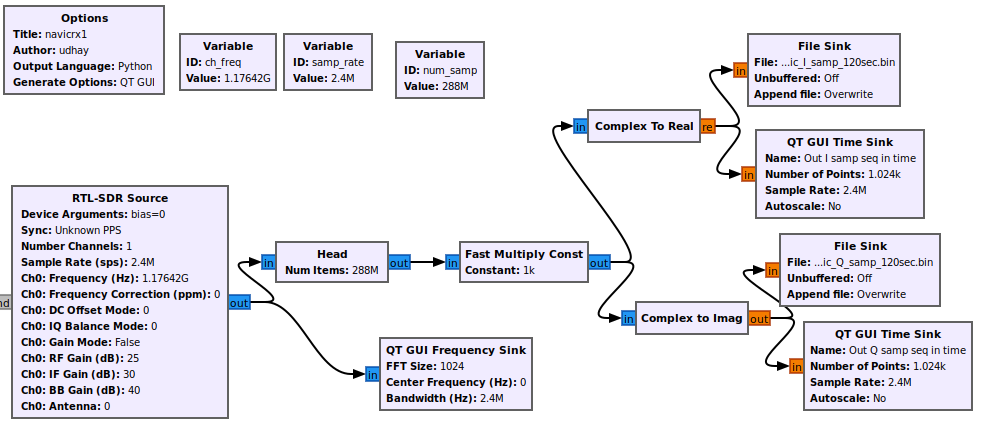
\includegraphics[scale=0.25]{figs/RTL_SDR_test.png} 
\end{align*}\\
\subsection{Results} 
\begin{align*}
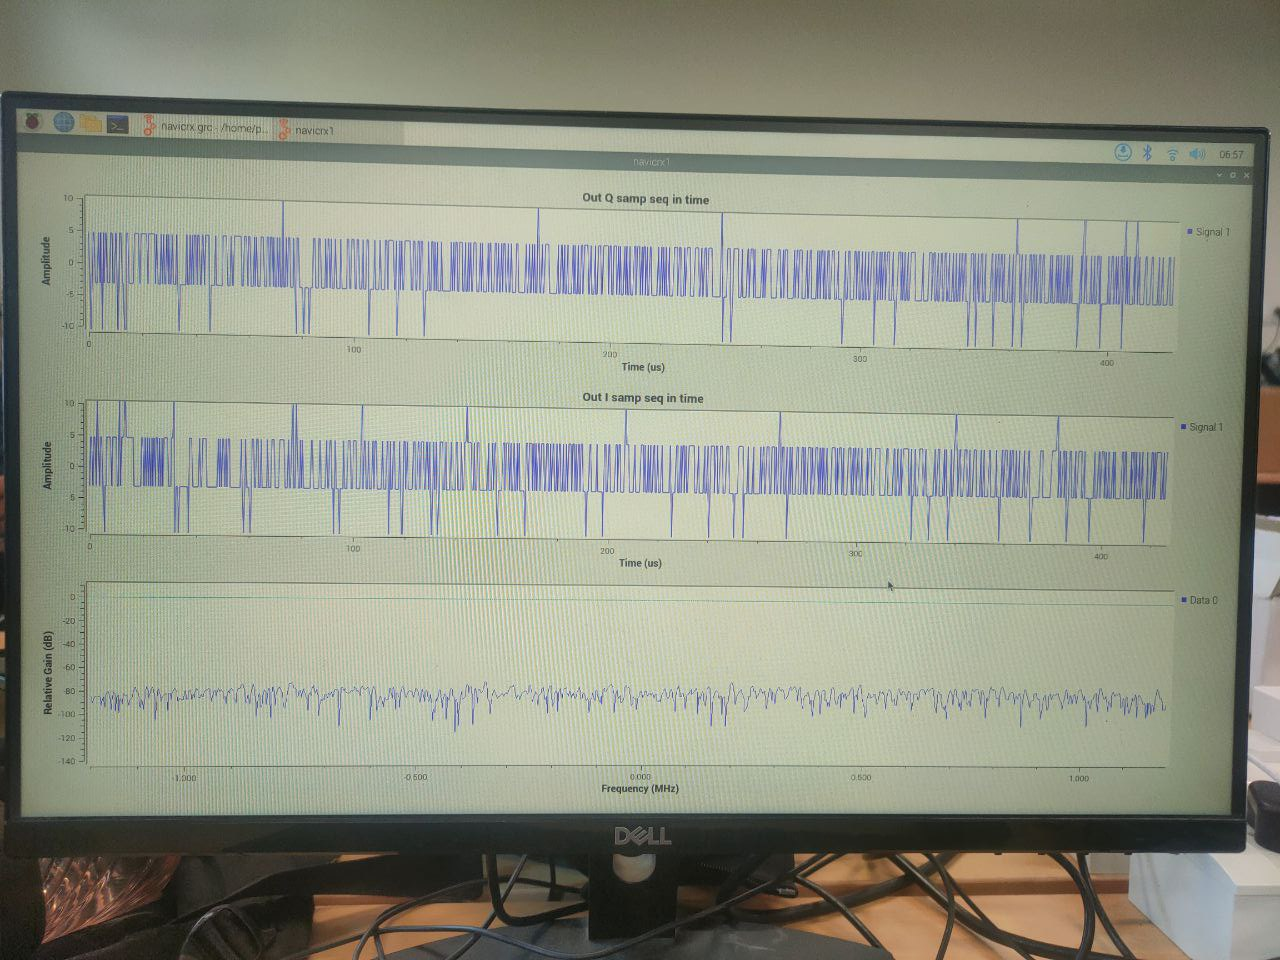
\includegraphics[scale=0.25]{figs/RTL_sdr_res.jpg} 
\end{align*}

\section{USRP SDR}
\subsection{SDR specification}
 \begin{tabular}{|c|c|}
	\hline
	\textbf{Name}&\textbf{USRP B210}\\
	\hline
	\textbf{Type}&\text{Pre-built}\\
	\hline
	\textbf{Frequency range}&\text{ 70 MHz – 6 GHz }\\
	\hline
	\textbf{Max. Bandwidth}&\text{56MHz }\\
	\hline
	\textbf{Receiver ADC bits}&\text{12}\\
		\hline
	\textbf{Tx. DAC bits}&\text{12}\\
	\hline
	\textbf{TX. Capable}&\text{Yes}\\
	\hline
	\textbf{Sampling Rate}&\text{56 Msps }\\
	\hline
	\textbf{Frequency accuracy ppm}&\text{-}\\
	\hline
	\textbf{Host interface}&\text{USB 3.0 }\\
	\hline
	\textbf{FPGA}&\text{Xilinx Spartan 6 XC6SLX150}\\
	\hline
\end{tabular}

\subsection{Radio block diagram for L5 band signal receiver}
\begin{align*}
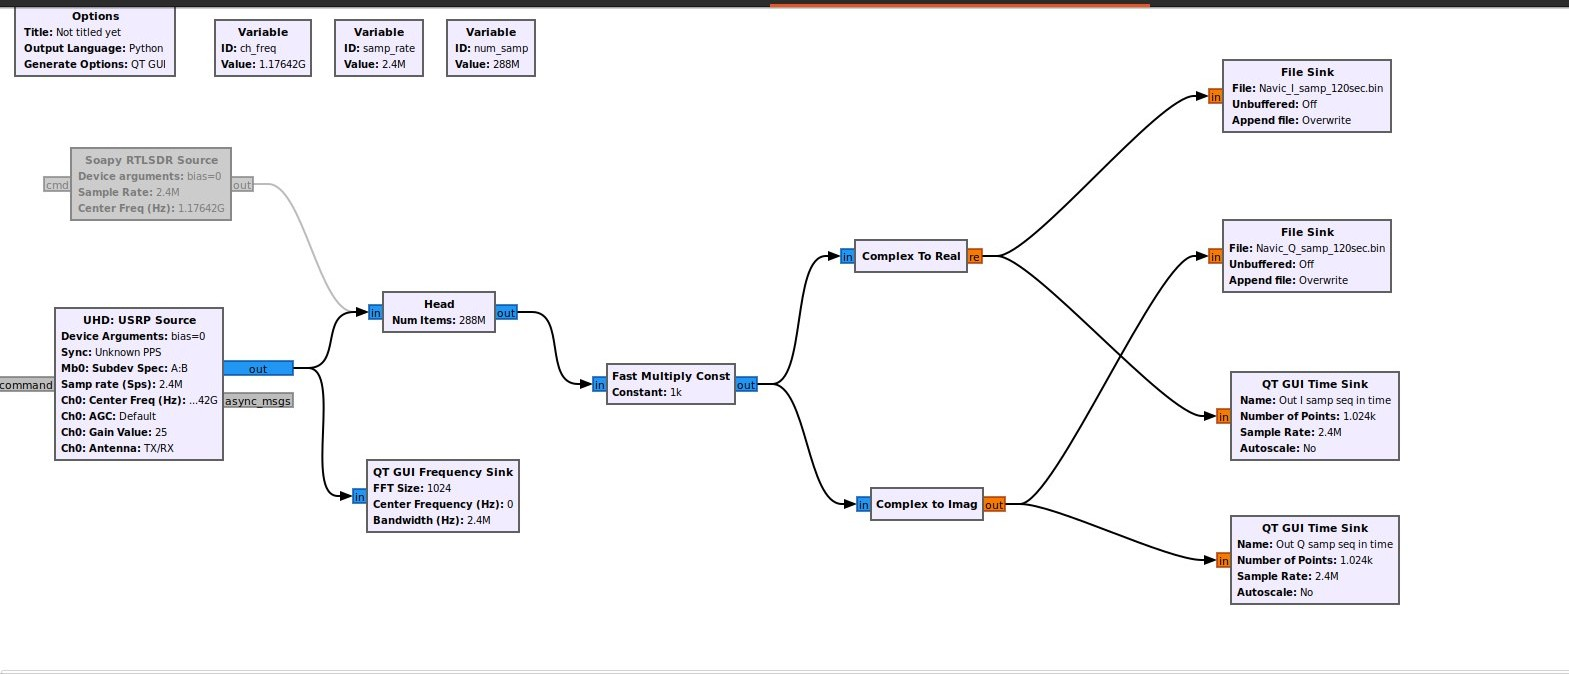
\includegraphics[scale=0.25]{figs/USRP_navic.jpg}  
\end{align*}\\
\subsection{Results} 
\begin{align*}
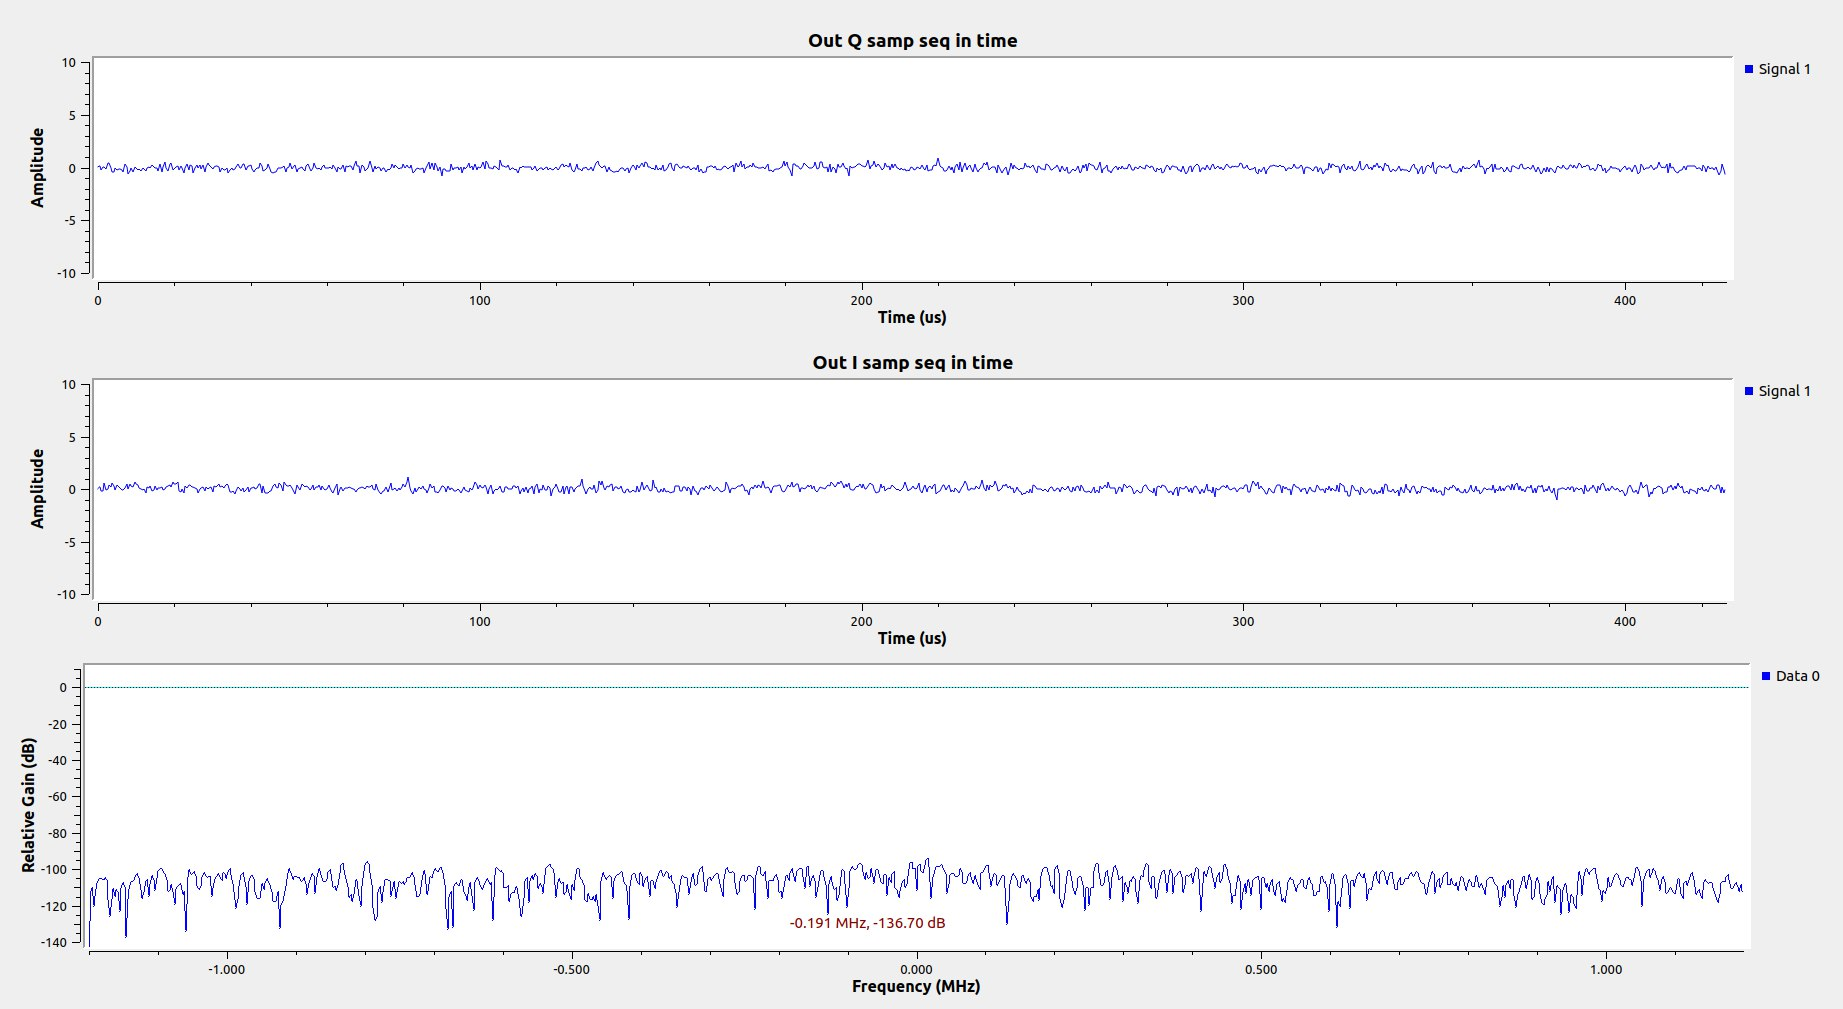
\includegraphics[scale=0.25]{figs/USRP_results.jpg}  
\end{align*}









\end{document} 
